\subsection{Qubits and Quantum States}
\label{subsec:qubits}

A \textit{qubit} is the fundamental unit of quantum information, represented as a normalized vector in a two-dimensional complex Hilbert space $\mathcal{H} = \mathbb{C}^2$. The standard basis states are:
\[
|0\rangle = \begin{pmatrix} 1 \\ 0 \end{pmatrix}, \quad |1\rangle = \begin{pmatrix} 0 \\ 1 \end{pmatrix}.
\]
A general qubit state is a superposition:
\[
|\psi\rangle = \alpha|0\rangle + \beta|1\rangle, \quad |\alpha|^2 + |\beta|^2 = 1,
\]
where $\alpha, \beta \in \mathbb{C}$ are probability amplitudes \cite{nielsen2010quantum}. This state can be visualized on the \textbf{Bloch sphere} (Figure \ref{fig:bloch_sphere}):
\[
|\psi\rangle = \cos\frac{\theta}{2}|0\rangle + e^{i\phi}\sin\frac{\theta}{2}|1\rangle,
\]
with $\theta \in [0, \pi]$ and $\phi \in [0, 2\pi)$.

\begin{figure}[h]
\centering
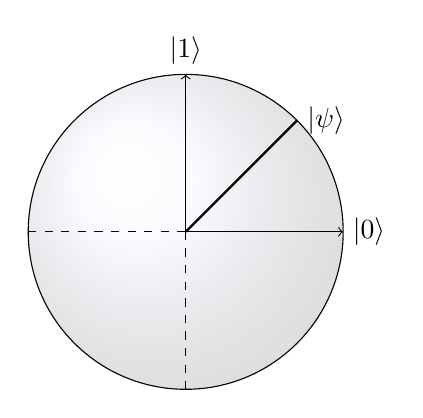
\begin{tikzpicture}
  \shade[ball color=blue!10!white,opacity=0.2] (0,0) circle (2cm);
  \draw (0,0) circle (2cm);
  \draw[thick] (0,0) -- (1.414,1.414) node[right] {$|\psi\rangle$};
  \draw[->] (0,0) -- (2,0) node[right] {$|0\rangle$};
  \draw[->] (0,0) -- (0,2) node[above] {$|1\rangle$};
  \draw[dashed] (0,0) -- (-2,0);
  \draw[dashed] (0,0) -- (0,-2);
\end{tikzpicture}
\caption{Bloch sphere representation of a qubit.}
\label{fig:bloch_sphere}
\end{figure}

For multi-qubit systems, the state space grows exponentially. A two-qubit system is described by:
\[
|\psi\rangle = \sum_{i,j \in \{0,1\}} \alpha_{ij}|i\rangle \otimes |j\rangle, \quad \sum_{i,j} |\alpha_{ij}|^2 = 1.
\]

\begin{table}[h]
\centering
\caption{Comparison of classical and quantum bits.}
\label{tab:qubit_vs_bit}
\begin{tabular}{|l|l|l|}
\hline
\textbf{Property} & \textbf{Classical Bit} & \textbf{Qubit} \\ \hline
State space       & $\{0, 1\}$            & $\mathbb{C}^2$ (superposition) \\ \hline
Measurement       & Deterministic         & Probabilistic (Born rule) \\ \hline
Entanglement      & N/A                   & Non-classical correlations \\ \hline
\end{tabular}
\end{table}